\chapter{Progettazione del sistema} %\label{1cap:spinta_laterale}
% [titolo ridotto se non ci dovesse stare] {titolo completo}
%

\begin{citazione}
In questo capitolo, trasformeremo i requisiti definiti nel capitolo precedente, in un progetto ben strutturato. Questo permetterà di costruire un sistema che non solo soddisfi le esigenze degli utenti, ma che sia anche robusto, scalabile e manutenibile nel tempo.
\end{citazione}
\newpage
\section{Progettazione dei test e scelta della metodologia}
Nel capitolo precedente sono stati definiti gli obiettivi che il presente studio intende raggiungere, oltre alle funzionalità che il sistema dovrà offrire a chi intende utilizzarlo. In questo capitolo saranno progettate le fasi utili al raggiungimento degli obiettivi prefissati partendo dalla definizione della \emph{metodologia} impiegata per l'ottenimento dei risultati sperati.
\subsection{Metodologia}
Per quanto riguarda i diversi esperimenti condotti con il sistema realizzato, è stato definito un \emph{flusso} di esecuzione univoco per tutti in modo da avere un metodo sperimentale da seguire, il quale aiuta a garantire che i risultati ottenuti siano affidabili e non siano dovuti al caso. Come rappresentato nella figura 4.1, ogni singolo esperimento si compone di diverse fasi:
\begin{itemize}
    \item Definizione del flusso di dati da testare;
    \item Invio del flusso tra client e server;
    \item Ottenimento output;
    \item Ripetizione del test 10 volte;
    \item Generazione dei grafici utilizzando gli output di ogni esecuzione.
\end{itemize}
Una volta definito il set di esperimenti ed i relativi flussi di dati aventi particolari requisiti di \emph{QoS}, esso sarà utilizzato in accoppiata con i protocolli \emph{WireGuard standard}, \emph{WireGuard post quantum}, \emph{OpenVPN} così da poter tirare fuori degli output sulla quale fare le dovute considerazioni.

\begin{figure}[h] 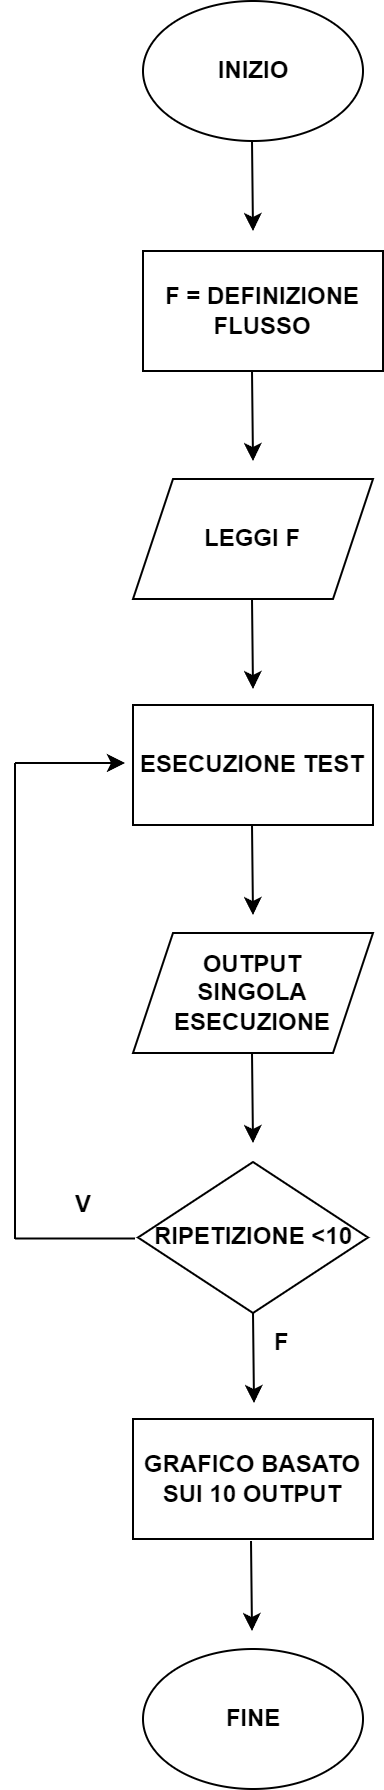
\includegraphics[width=0.2\textwidth] {Tesi magistrale/capitoli/images/flow.png}
\centering
\caption{Flusso di esecuzione degli esperimenti.}
\end{figure}

\newpage
\section{Architettura del sistema}
L'architettura del sistema è fondamentale per comprendere come esso funzioni nel suo insieme e come le sue parti interagiscono tra loro. Nel contesto di questo progetto, \emph{l'architettura fisica} è organizzata come rappresentato nella figura 4.2; il dispositivo realizzato sarà collocato all'interno di una qualsiasi rete LAN e permetterà, ai diversi client che vogliono accedere alla medesima LAN, di poterlo fare tramite la connessione ad un canale VPN realizzato con WireGuard.
\begin{figure}[h] 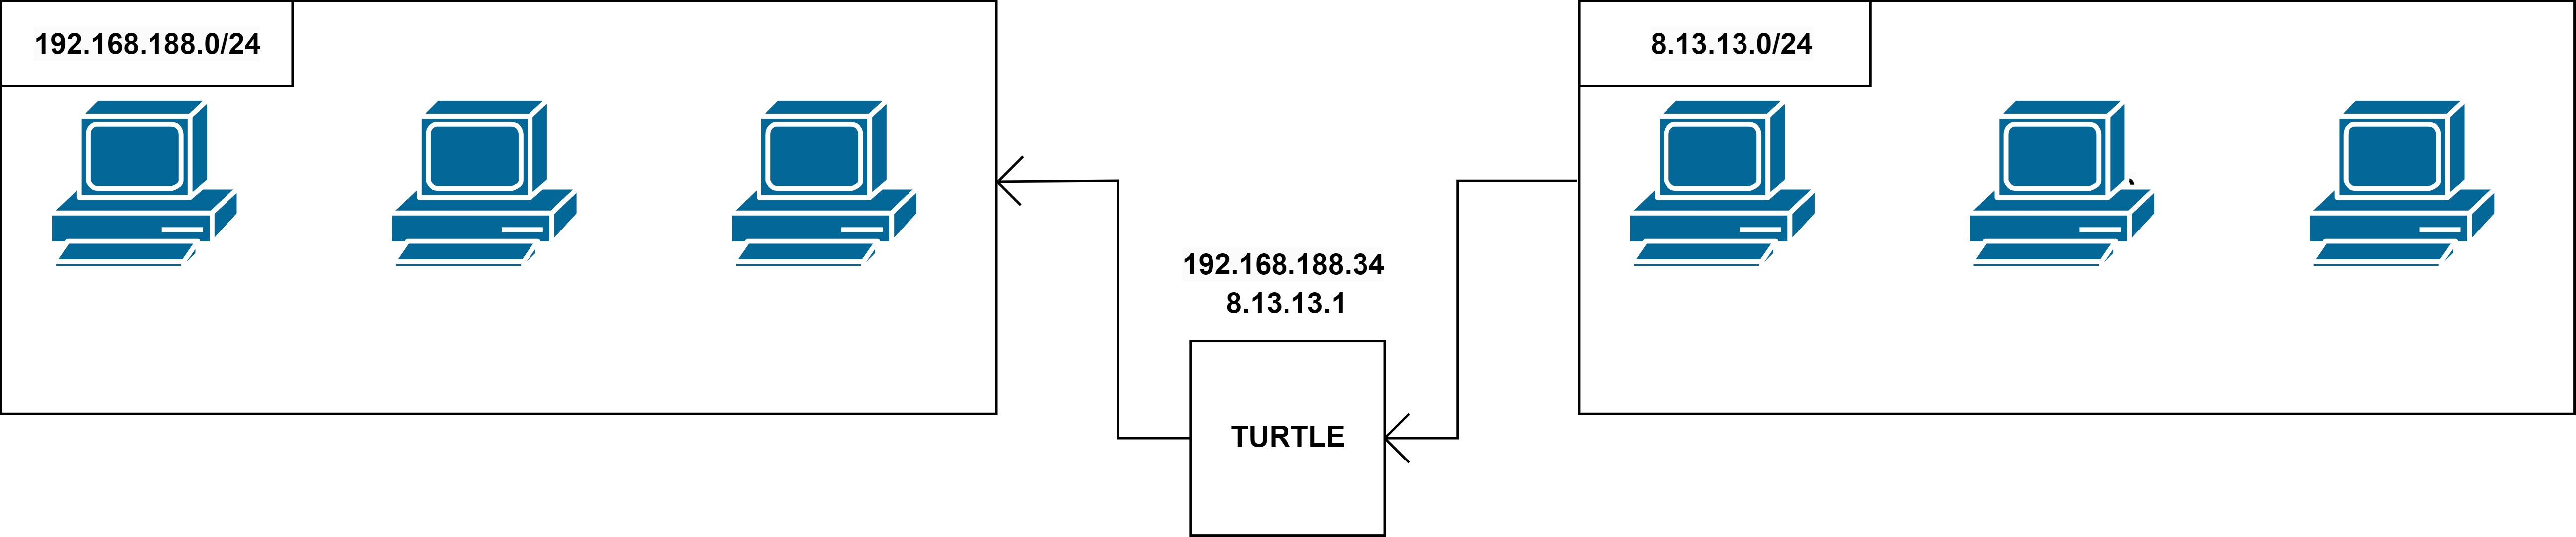
\includegraphics[width=1\textwidth] {Tesi magistrale/capitoli/images/Schema turtle.png}
\centering
\caption{Schema TurtleVPN.}
\end{figure}


\section{Progettazione hardware}
La scelta dei componenti \emph{hardware} è un passaggio fondamentale in qualsiasi progetto e ancor di più in questo; essa influenzerà le prestazioni di tutto il sistemata per cui è molto importante scegliere le componenti adeguate anche in base alle performance che si vogliono ottenere, soprattutto per garantire una buona \emph{stabilità} e \emph{connettività} agli utenti finali. Alla base del sistema da realizzare è stata impiegata la scheda \emph{Raspberry Pi 4 model B} \cite{rasp}.
\begin{figure}[h] 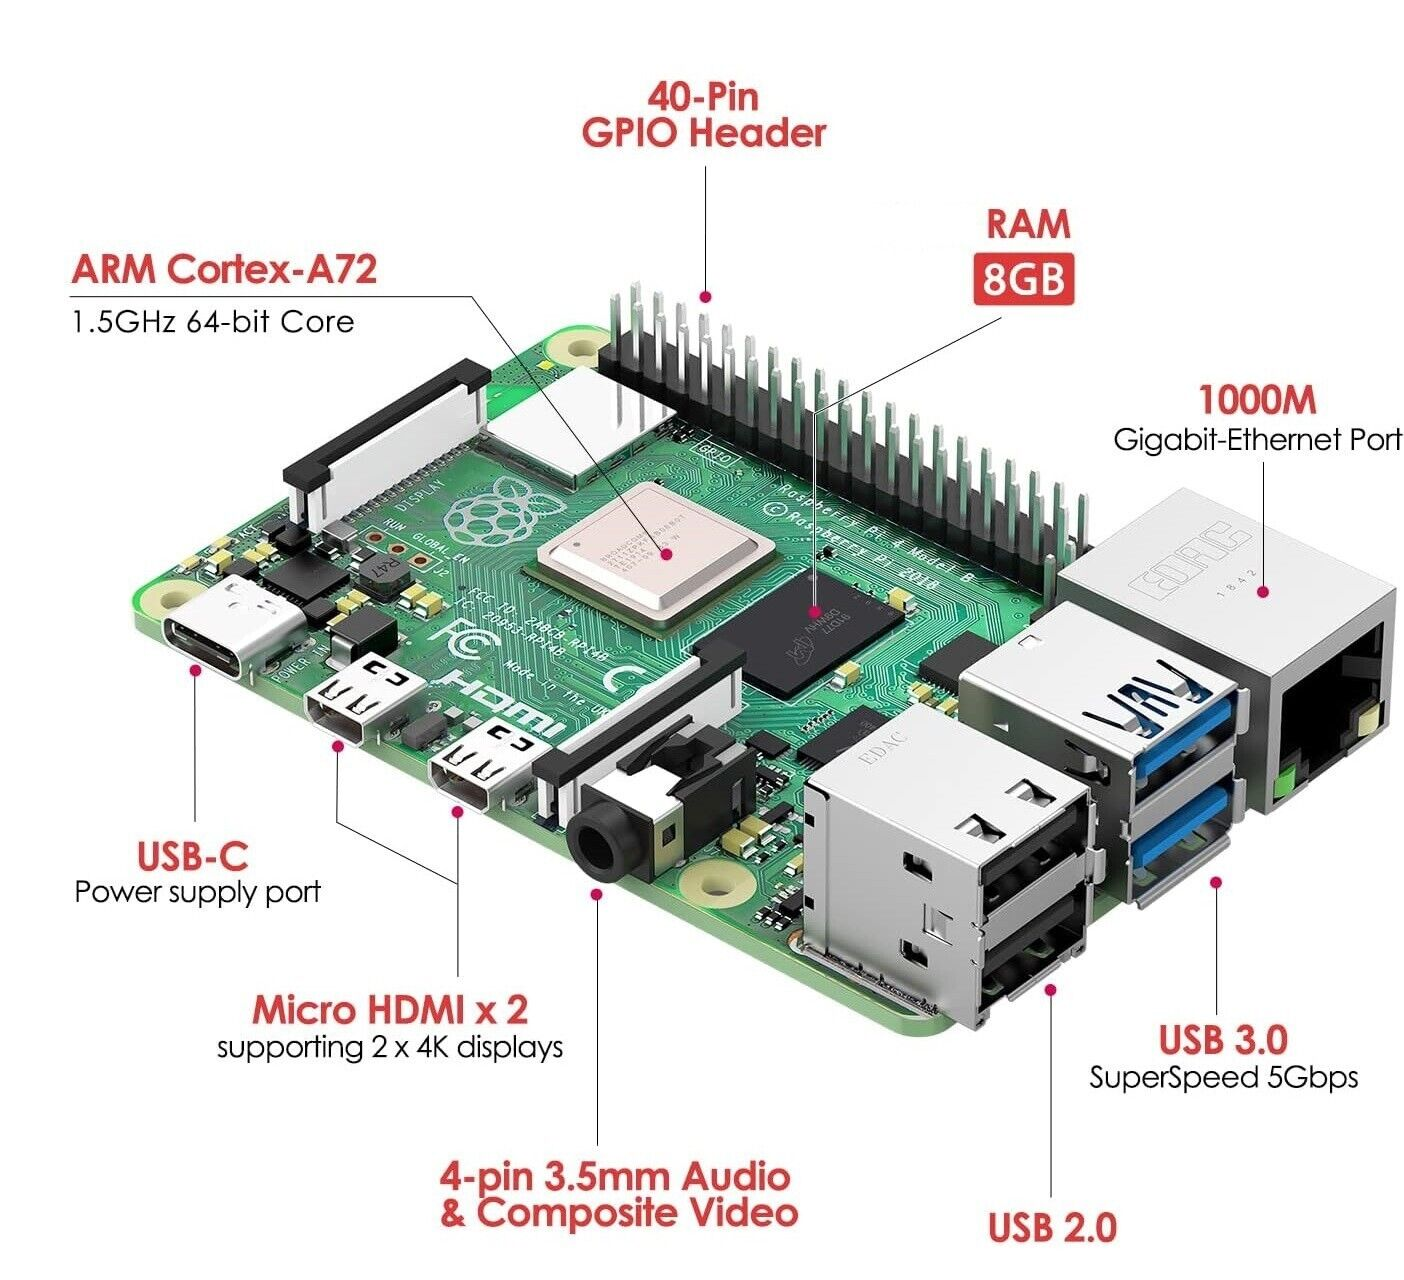
\includegraphics[width=0.6\textwidth] {Tesi magistrale/capitoli/images/rasp.jpg}
\centering
\caption{Raspberry Pi 4 model B.}
\end{figure}

\subsection{Architettura del dispositivo Raspberry Pi}
Il sistema ideato sarà implementato a partire dalla scheda one board \emph{Raspberry Pi 4 model B} che offre la possibilità di poter installare diversi sistemi operativi \emph{Linux based}. Tale scheda ha delle prestazioni molto simili ad un normale computer di fascia entry-level permettendo così di adempire in modo adeguato ai compiti stabiliti. 
\begin{itemize}
    \item Processore quad-core a 64 bit
    \item 8GB di RAM
    \item Decodifica hardware video fino a 4Kp60
    \item Dual-band 2.4 /5.0 GHz LAN wireless
    \item Gigabit Ethernet
    \item Bluetooth 5.0
    \item USB 3.0
\end{itemize}

\subsection{Scelta del sistema operativo}
Per quanto riguarda la scelta del sistema operativo, ne esistono di svariati tra cui \emph{Raspbian}, \emph{Ubuntu MATE}, \emph{Arch Linux} ma per questo progetto è stato utilizzato \emph{Ubuntu Server} versione \emph{22.04.3 LTS} il quale offre sicuramente ottima stabilità e costanza negli aggiornamenti per lungo tempo.

\section{Progettazione software}
Passiamo ora alla progettazione delle funzionalità stabilite. Esse saranno organizzate in diversi \emph{moduli} ognuno dei quali sarà completamente indipendente e funzionante in autonomia. Prima di procedere è necessaria eseguire l'installazione del sistema operativo sulla scheda in questione.

\subsection{Installazione del sistema operativo}
L'installazione del sistema operativo sulla scheda Raspberry Pi 4 è stata eseguita utilizzando l'ottimo tool \emph{Pi imager} il quale offre la possibilità di poter scaricare un sistema operativo compatibile con una delle schede Raspberry e di automatizzare il processo di installazione di esso.
\begin{figure}[h] 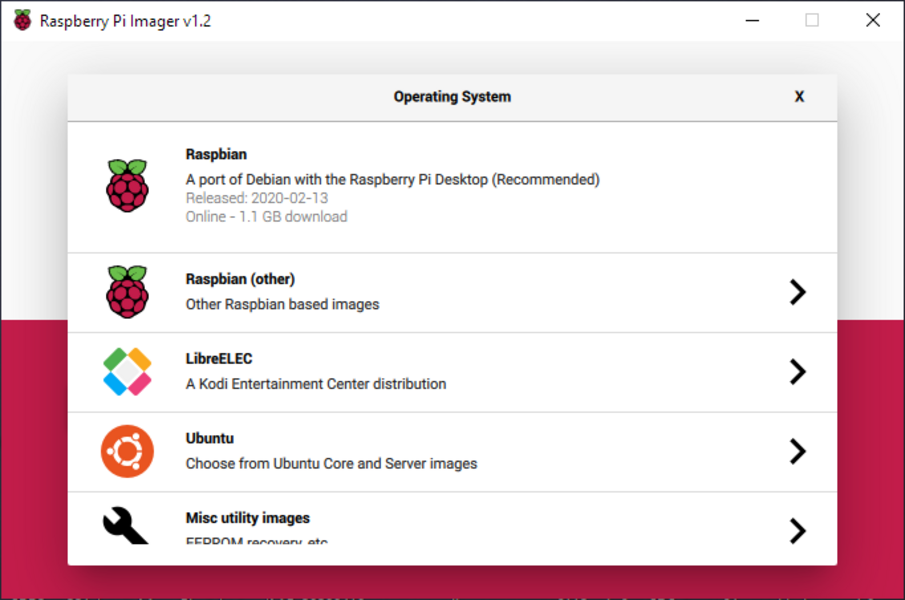
\includegraphics[width=0.5\textwidth] {Tesi magistrale/capitoli/images/pi imager.png}
\centering
\caption{Raspberry Pi imager.}
\end{figure}
\newpage

\subsection{Integrazione di Nmap per le scansioni di rete}
Il primo modulo è stato progettato con lo scopo di fornire all'utente finale la possibilità di effettuare diverse tipologie di scansione all'interno della rete in modo da poter acquisire facilmente importanti informazioni sugli \emph{host} presenti in essa. Per soddisfare tale compito è stato scelto di utilizzare il noto network scanner \emph{Nmap} \cite{nm}. Per quanto riguarda la realizzazione del modulo in sé è stato scelto di impiegare il linguaggio di programmazione \emph{Python} \cite{py} il quale al giorno d'oggi rappresenta sicuramente uno dei linguaggi più versatili, avente un gran numero di \emph{librerie} a disposizione.

\subsubsection{Gestione delle richieste HTTP}
Le diverse scansioni realizzate tramite l'utilizzo di \emph{Nmap} e \emph{Python} saranno poi rese accessibili ai diversi utilizzatori grazie all'impiego del framework \emph{Flask} \cite{fl} il quale rappresenta un ottima scelta per quanto riguarda la programmazione web \emph{backend}. Con tale framework saranno implementate diverse funzioni che possono gestire le richieste HTTP in arrivo dai client.


\subsection{Integrazione dei servizi VPN}
Il secondo modulo è stato progettato con l'obiettivo di fornire agli utenti la possibilità di connettersi ad un \emph{server VPN} il quale instaura un canale cifrato tra il client che usufruisce del servizio e la rete LAN a cui è connesso il dispositivo Raspberry Pi 4, in modo che tale client entri a far parte di quella rete e possa avere accesso alle \emph{risorse} presenti all'interno di essa. Per assolvere a questo compito è stato scelto di utilizzare il protocollo \emph{WireGuard VPN} versione \emph{standard} \cite{wir} il quale risulta essere molto semplice da configurare ma allo stesso tempo offre ottime prestazioni, superiori anche al protocollo \emph{OpenVPN} \cite{op}.
